\chapter{Overview}%
\label{ch:overview}%


In this chapter, we give an overview of the contributions of this dissertation.
This shall serve both as an introduction and as a high-level summary of the detailed explanations in the following chapters.
All contributions can be located in the research area of design time analysis and architecture-based quality prediction \cite{reussner_modeling_2016}.
Here, common benefits are simplifying the work of software architects and enhancing existing analysis approaches, e.g., regarding their applicability, scalability, accuracy, or usability \cite{konersmann_evaluation_2022}.

The central research concern of this thesis is confidentiality analysis under uncertainty by using architectural modeling \cite{hahner_dealing_2021}.
We divide the contributions of this thesis into three parts:
First, the identification and classification of uncertainty regarding confidentiality.
Second, the uncertainty impact analysis by propagating uncertainty within architectural models and data flow diagrams.
Third, the architecture-based confidentiality analysis under uncertainty.
Each of these contributions can be used independently and enhances the state of the art in its area.
However, they can also be combined to form a comprehensive end-to-end approach which is an aspired goal in the community \cite{weyns_towards_2023,hezavehi_uncertainty_2021}.

In the following, we describe the general procedure for uncertainty-aware analyses and how our contributions are positioned within it.
We briefly introduce these contributions afterward.
Last, we give an overview of the tool support that has been developed to complement the research.

\ownpublications{
\fancycite{hahner_dealing_2021}, 
\fancycite{hahner_architectural_2021}, 
\fancycite{acosta_uncertainty_2022}, 
\fancycite{hahner_model-based_2023}, 
\fancycite{hahner_classification_2023},
\fancycite{camara_uncertainty_2024},
\fancycite{hahner_arcn_2024}
}





\section{Procedure for Uncertainty-Aware Analyses}%
\label{sec:overview:procedure}

Incorporating uncertainty in the analysis of software systems---thus achieving uncertainty awareness---has been discussed within the literature \cite{garlan_software_2010,sobhy_evaluation_2021,troya_uncertainty_2021}.
\textcite{garlan_software_2010} proposed to include uncertainty as \enquote{first-class concern in the design, implementation, and deployment} of software systems.
\textcite{hezavehi_uncertainty_2021} conducted a community survey and proposed a reference process for uncertainty management.
They include phases like identification, modeling, impact analysis, and assessment.
However, their process aims at \acfp{SAS} that include run time strategies that are beyond the scope of this thesis.
Regarding model-based analyses at design time \cite{acosta_uncertainty_2022}, we consider four central activities: 

\begin{enumerate}
    \item \textbf{Identification and awareness}: 
    To include uncertainty sources in the analysis, they must be known first.
    Thus, raising awareness to recognize the presence of uncertainty in a system is the necessary first step.

    \item \textbf{Classification}: 
    To better understand the type of uncertainty sources and their properties, they can be classified.
    To that end, classifications and taxonomies provide the foundations for the documentation and the discussion of identified uncertainty.

    \item \textbf{Propagation}: To assess the impact of identified and classified uncertainty sources, they can be propagated through the architectural model.
    Estimating the potential impact early helps in making more precise statements and decisions.

    \item \textbf{Analysis}: To apply appropriate mitigation strategies, the effect of uncertainty on the software system's quality has to be analyzed.
    In our case, this means identifying confidentiality violations due to the identified, classified, and propagated uncertainty.
\end{enumerate}

\begin{figure}
    \centering
    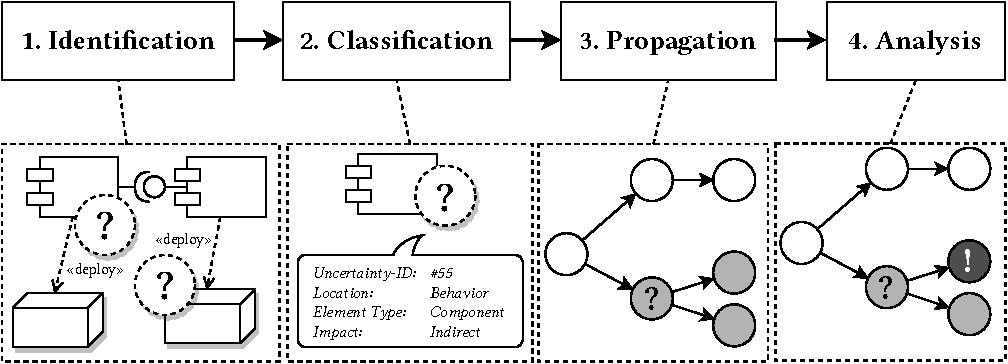
\includegraphics[width=\textwidth]{figures/chapter4/overview-informal.pdf}
    \caption{Informal overview of the central activities of uncertainty-aware analyses}
    \label{fig:overview:informal}
\end{figure}

\autoref{fig:overview:informal} illustrates these four activities in an informal diagram.
\emph{First}, uncertainty sources have to be identified, e.g., within the software system or its environment.
In \autoref{fig:overview:informal}, we annotate these uncertainty sources in the architectural model similar to the running example presented in \autoref{ch:runningexample}.
In the \emph{second} activity, these uncertainty sources have to be described according to an appropriate classification \cite{hahner_classification_2023}.
This does not only help in the understanding of the underlying problem but also enables an uniform handling in the later activities.
The \emph{third} activity is the propagation of uncertainty sources to estimate their potential impact.
Here, software architects develop an understanding of which parts of the software systems could be affected and which parts can be safely ignored.
The \emph{fourth} activity is the confidentiality analysis under uncertainty.
This activity yields confidentiality violations in those parts of the software system that have been impacted by uncertainty.

\finding{Literature proposed processes for uncertainty management.
Common steps are the identification, classification, propagation, and analysis of uncertainty.
By applying these activities to confidentiality analysis, we can provide a comprehensive approach to identify confidentiality violations under uncertainty.}

A high-level description like the informal overview introduced in \autoref{fig:overview:informal} serves as an overview or introduction.
However, due to the high abstraction, two important details are left out.
\emph{First}, the procedure does not need to be linear.
Sometimes, not all activities are required, e.g., because a critical subsystem has to be always analyzed despite the results of the propagation.
Additionally, some activities or the procedure might be repeated, either because of the understanding of the uncertainty or because the system evolves \cite{weyns_towards_2023}.
Especially with regard to uncertainty and \acp{SAS}, approaches tend to be iterative and incremental, as in continuous architecture evaluation \cite{sobhy_evaluation_2021}, or in the \acf{MAPEK} loop \cite{kephart_vision_2003,weyns_patterns_2013}.
\emph{Second}, the informal overview lacks role descriptions.
Specifying expertise and required knowledge helps in understanding the application of analysis procedures.

\begin{figure}
    \centering
    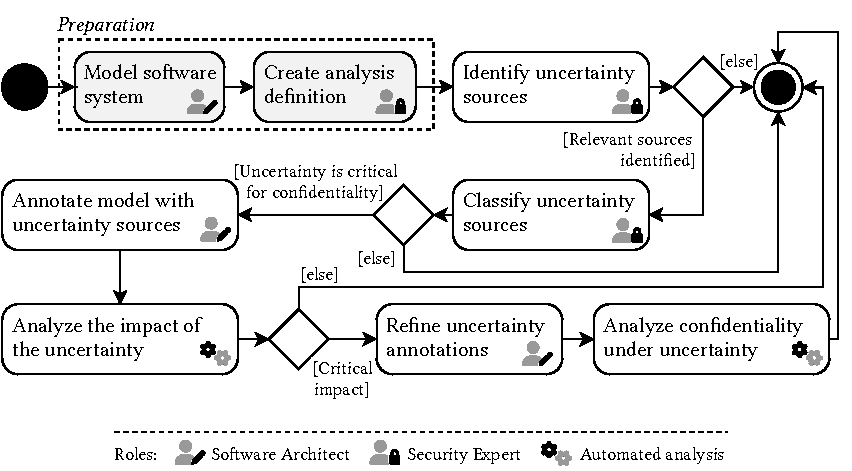
\includegraphics[width=\textwidth]{figures/chapter4/overview-procedure.pdf}
    \caption{Proposed analysis procedure showing the modeling and analysis activities and assigned roles.}
    \label{fig:overview:procedure}
\end{figure}

To address these shortcomings, we provide a more detailed procedure with \autoref{fig:overview:procedure}.
We reuse the roles proposed for architectural confidentiality analysis \cite{seifermann_architectural_2022}, i.e., \emph{software architect} and \emph{security expert}.
Note, that we do not introduce a role for \emph{uncertainty experts}.
With appropriate means like tool-supported identification, classification, and analysis approaches, only minimal additional knowledge shall be required.
Thus, we do require expert knowledge of uncertainty classification or uncertainty sources in general.

The procedure starts with the preparation phase which comprises modeling the software system \cite{seifermann_data-driven_2019,seifermann_identifying_2021} and creating the analysis definition \cite{hahner_modeling_2021}.
These steps originate from architectural data flow analysis \cite{seifermann_architectural_2022}.
An architectural model has to be defined by a software architect using an \acf{ADL} like the \acf{PCM} or \acfp{DFD}.
Afterward, confidentiality requirements serve as input for the security expert to create the confidentiality analysis definition.
This enables identifying confidentiality violations without considering uncertainty.

First, uncertainty sources have to be identified by the security expert.
Although we do not require expert knowledge of uncertainty, security expertise helps estimate the potential impact on confidentiality.
Uncertainty sources can be identified in discussions, architecture reviews, or using checklists, guidelines, or catalogs \cite{hahner_arcn_2024}. 
If no relevant sources have been identified, the procedure ends until new knowledge about uncertainty is gained.
This step represents the first activity of identification and awareness. 

In the next step, the identified uncertainty sources are classified according to an appropriate classification \cite{hahner_classification_2023}.
This step is performed by the security expert with the help of existing catalogs that bootstrap the classification.
If only uncertainty sources have been identified that clearly have no impact on confidentiality, the procedure ends.
This step represents the second activity.
Based on the result of the classification, the uncertainty sources are annotated to the architectural model.
This does not require security expertise but knowledge of the \ac{ADL} in use and is thus driven by the software architect.

Afterward, the uncertainty impact analysis propagates the uncertainty source within the software system and calculates the potential impact \cite{hahner_architecture-based_2023}.
This step represents the third activity and is fully automated and thus requires neither knowledge about security nor software architecture.
If no relevant uncertainty impact is identified, e.g., because only non-critical parts of a software system are affected, the procedure ends.
Otherwise, the confidentiality under uncertainty has to be analyzed which is the fourth activity.
This includes a more detailed specification of the uncertainty sources for a precise analysis result.
While the refinement of the information about the uncertainty is conducted by the software architect, the analysis is fully automated.
Afterward, the procedure ends.

Note that the end of the procedure does not imply the end of the design and analysis process.
If the knowledge about uncertainty or the software systems changes, the procedure can be restarted.
Additionally, all artefacts like the modeled software architecture, the analysis definition, collected uncertainty sources and their classification and annotation can be reused.
Thus, we consider this procedure to be iterative.
As stated previously, we do not require expert knowledge about uncertainty.
The classification and the automated analyses, i.e., the uncertainty impact analysis and the uncertainty-aware confidentiality analysis encapsulate the required knowledge \cite{hahner_model-based_2023}.
The procedure has to be incremental as the existence of uncertainty is inherent to software systems.
It can never be assured to be aware of all uncertainty sources, as \emph{unknown unknowns} \cite{perez-palacin_uncertainties_2014} might exist.
In this way, uncertainty is similar to bugs in software systems, where testing can only be used to show the \enquote{presence of bugs, but never to show their absence} \cite{dijkstra_notes_1970}.
Additionally, the procedure requires exit points after each activity when more knowledge is gained about the impact of uncertainty on the software system's confidentiality.

\finding{Due to the nature of uncertainty, it is impossible to ensure its absence.
However, not every uncertainty source causes confidentiality violations.
This depends on many aspects like the uncertainty itself, confidentiality requirements, security measures, or the software's architecture.
A procedure for uncertainty-aware confidentiality analysis has to be iterative and incremental.}





\section{Overview of the Contributions}%
\label{sec:overview:contributions}

In the following, we introduce the central contributions of this thesis and relate them to the procedure presented hereabove.
We divide the contributions into three main parts:

\begin{enumerate}[label=\textbf{C\arabic*}]
    \item \textbf{Identification and classification}: Recognizing and understanding the types of uncertainty and their relation to confidentiality from an architectural point of view.
    \item \textbf{Uncertainty impact analysis}: Propagating uncertainty using architectural models and \acp{DFD} to predict the uncertainty impact on the system's confidentiality.
    \item \textbf{Uncertainty-aware confidentiality analysis}: Extending architecture-based confidentiality analysis to consider uncertainty as a first-class concern in both modeling and analysis to identify confidentiality violations under uncertainty.
\end{enumerate}

First, with Contribution \C{1}, we aim to support software architects in identifying and classifying relevant uncertainty sources with a potential impact on confidentiality.
This is an elemental first step, as awareness about uncertainty sources and their properties is key in documentation, modeling, discussion, and analysis \cite{garlan_unknown_2021}.
This combines the activities of identification and classification in one contribution, as both are interdependent and support each other.
We contribute a classification of software-architectural uncertainty \cite{hahner_classification_2023} and support the collaborative identification of uncertainty sources \cite{hahner_arcn_2024}.
During this research, we also examine \acfp{CPS} as a relevant type of uncertainty-afflicted software systems \cite{acosta_uncertainty_2022}.
Our findings answer \RQ{1}, which is related to the identification and description of uncertainty with regard to confidentiality.

Our second Contribution \C{2} addresses the impact analysis of uncertainty, which supports the early prediction and assessment of the uncertainty impact.
Similar to change impact analysis \cite{rostami_architecture-based_2015,rostami_architecture-based_2017}, we propagate uncertainty through the software architecture.
Besides the theoretical foundations of modeling and propagating uncertainty in architectural models and \acp{DFD}, this contribution also includes a fully automated analysis \cite{hahner_architecture-based_2023}.
Based on our concept of uncertainty propagation in \acp{DFD}, additional research led to the formulation of \acp{UFD} \cite{camara_uncertainty_2024}.
They support software architects in understanding and analyzing uncertainty interactions \cite{camara_addressing_2022}.
In sum, these findings provide an answer to \RQ{2}, which relates to architectural uncertainty propagation and impact analysis.

In our third Contribution \C{3}, we develop confidentiality analysis approaches that respect uncertainty.
To that end, we extend an existing architecture-based confidentiality analysis which utilizes \acp{DFD} \cite{seifermann_architectural_2022,seifermann_detecting_2022}.
We provide approaches for different types of uncertainty, e.g., environmental uncertainty \cite{boltz_handling_2022}, or structural uncertainty \cite{walter_architectural_2022}.
By defining an analysis framework for architectural data flow analysis, we also provide the baseline for more comprehensive approaches \cite{boltz_extensible_2024}.
We use this framework to research the expressiveness, accuracy, and scalability of data flow-based confidentiality analysis under uncertainty \cite{hahner_model-based_2023}.
These approaches address \RQ{3}, which asks how to consider uncertainty in architectural confidentiality analysis. 





\section{Tool Support}%
\label{sec:overview:toolsupport}

In addition to answering the research questions of this thesis, we provide comprehensive tool support.
For each contribution, we realized tooling to demonstrate the applicability of the concepts.
The prototypical implementation is not only used in the evaluation but also shall support further research \cite{boltz_extensible_2024}.
A recent \acf{SLR} found a lack of replication packages in software architecture research \cite{konersmann_evaluation_2022}.
To address this, all tool support is open source, publicly available and also part of this thesis' data set \cite{dataset}.

Automated analyses support software architects because they encapsulate expert knowledge, e.g., annotation and propagation rules \cite{hahner_classification_2023}.
Especially in large software systems or systems of systems, manual analysis is also not feasible and error-prone \cite{seifermann_data-driven_2019}.
In our iterative procedure, it cannot be assumed that software architects manually evaluate hundreds of \ac{DFD} nodes \cite{hahner_classification_2023} without mistakes.
Additionally, after each change to the annotated uncertainty sources or the software system, the manual work would have to start all over again.
Thus, it is important to ensure that the developed concepts can be automated to a high degree without manual effort required from software architects.
Similar to the division into three contributions, we provide three tooling artifacts.
We introduce and shortly summarize their functionality in the following%
\footnote{At the time of writing---and hopefully a long time to come---the most up-to-date version of all tool support is online available here: \url{https://abunai.dev/}. Once the link is broken, please refer to the data set \cite{dataset}.}.

\arcen stands for rese\uff{arc}h \uff{arc}hive for Software-\uff{arc}hitectural u\uff{n}certainty.
This is a web-based interactive catalog of uncertainty sources that can affect confidentiality \cite{hahner_arcn_2024}.
It simplifies the identification by connecting a classification \cite{hahner_classification_2023} to a catalog approach.
All data is publicly available, extensible by other researchers, and can be integrated into existing analyses.
This catalog of uncertainty sources supports Contribution \C{1}.

\uia means \uff{u}ncertainty \uff{i}mpact \uff{a}nalysis and is a tool for propagating uncertainty sources within architectural models and \acp{DFD}.
It extends the data flow analysis framework \cite{boltz_extensible_2024}.
The tool support is realized as an Eclipse plugin and can be integrated into the existing Palladio tooling \cite{reussner_modeling_2016}.
The analysis yields an impact set for uncertainty sources which can be annotated to the software architecture.
Besides the annotation, no additional effort is required for existing \ac{PCM} models as the propagation is fully automated.
See \autoref{sec:appendix:impactset} for an exemplary impact analysis result.
This supports our second Contribution \C{2}.

\abunai is short for \uff{a}rchitecture-\uff{b}ased and \uff{un}certainty-\uff{a}ware confidentiality analys\uff{i}s\footnote{Furthermore, the Japanese word \emph{abunai} translates to dangerous, risky, or uncertain. How fitting!}.
Similarly to the uncertainty impact analysis, this tooling is realized as an Eclipse plugin and extends the data flow analysis framework \cite{boltz_extensible_2024} within the Palladio approach \cite{reussner_modeling_2016}.
This analysis enables software architects to refine the uncertainty annotations by providing possible scenarios \cite{hahner_model-based_2023}.
Afterward, the automated analysis considers the uncertainty impact in the data flow analysis and yields confidentiality violations with respect to uncertainty.
See \autoref{sec:appendix:runningexample} and \autoref{sec:appendix:confidentiality} for exemplary analysis inputs and analysis results.
This is one of the analysis approaches that support Contribution \C{3}.





\section{Illustration using the Running Example}%
\label{sec:overview:illustration}

We demonstrate the procedure, the contributions, and the tool support briefly using the running example introduced in \autoref{ch:runningexample}.
We assume a team of software architects and security experts that already modeled the software system using \ac{PCM} and created the analysis definition to analyze the system's confidentiality.
See the preparation phase in \autoref{sec:overview:procedure} for more details.

First, relevant uncertainty sources have to be identified by security experts.
As part of our first Contribution \C{1}, the tool support \arcen provides a catalog of uncertainty sources that serve as a starting point.
The catalog also contains all uncertainty sources which have been annotated to the running example, e.g., the user input (\U{1}), or the provider's trustworthiness (\U{4}).
As the uncertainty sources in this catalog already are classified, the subsequent step of uncertainty classification is simplified or can be skipped.
All of the contained sources are relevant regarding confidentiality.
The software architect annotates the uncertainty sources within the architectural model in the running example.
For example, the user input uncertainty (\U{1}) is annotated to the \emph{Customer}, and the data processing uncertainty (\U{2}) is annotated to the \emph{Online Shop} component.
In \autoref{fig:runningexample:architecture}, we illustrate this annotation using circled question marks.

Using the architectural models and the annotations as input, the impact analysis calculates the potential impact on confidentiality.
This is part of our second Contribution \C{2}, and fully automated with \uia.
In the running example, the impact set of all uncertainty sources contains the \emph{Database Service} component.
As the database stores confidential data, we interpret this impact as being critical continue with the step of uncertainty source refinement.
The precise modeling of uncertainty sources and scenarios and the analysis are part of our third Contribution \C{3}.
In the running example, the software architects describe all relevant scenarios, e.g., the possible deployment locations of the \emph{On Premise Server} or the \emph{Cloud Service}.
Afterward, the automated analysis \abunai yields confidentiality violations due to single or multiple uncertainty scenarios.
In our running example, the lack of proper data processing (\U{2}) and the deployment in the cloud (\U{3}) without proper security measures violate confidentiality.
After addressing these issues, the procedure can be repeated.
This also happens whenever the software system changes, e.g., due to the introduction of a new encryption component, or the knowledge about the uncertainty changes, e.g., because the scenario of the lack of any data processing can be excluded.





\section{Summary and Outlook}%
\label{sec:overview:summary}

In this chapter, we discussed the procedure of uncertainty-aware analysis and summarized the contributions of this thesis.
First, we investigated multiple proposals for required activities in uncertainty-aware analysis.
We combined them to propose a procedure for architecture-based confidentiality analysis under uncertainty.
This procedure contains the central activities of identification, classification, propagation, and analysis.
Besides these activities, our proposed procedure also contains modeling activities carried out by software architects and security experts.
The analyses are fully automated and thus shall not require additional knowledge about uncertainty.
The procedure is both iterative and incremental to react to changes in the system, its environment, and its uncertainty sources.
Put simply, uncertainty is uncertain, and we have to deal with it.

Afterward, we gave an overview of the central contributions of this thesis.
They cover the aforementioned activities of identification and classification with Contribution \C{1}, the propagation and uncertainty impact analysis with Contribution \C{2}, and the uncertainty-aware confidentiality analysis with Contribution \C{3}.
All contributions are tool-supported with three research artifacts: \arcen collects and explains uncertainty sources and their classification, \uia automatically propagates uncertainty in an architectural model to calculate the potential impact, and \abunai provides uncertainty-aware confidentiality analysis based on architectural modeling and \acp{DFD}.
Last, we illustrated the tool-supported contributions and their interrelationships using the running example.
The application of our prototypical tooling is also shown in \autoref{sec:appendix:runningexample}, \autoref{sec:appendix:impactset}, and \autoref{sec:appendix:confidentiality}.

Throughout this chapter, we stressed the lack of an explicit role for uncertainty experts in the proposed procedure.
Ideally, automated analyses and other artifacts should encapsulate the required knowledge about uncertainty.
We will return to this idea in the following chapters and explain the consequences in more detail.
The illustration in this chapter was based on \readingpath{ch:runningexample}.
In the following three chapters, we present the contributions in detail.
In \readingpath{ch:classification}, we show the first Contribution \C{1}, in \readingpath{ch:impactanalysis}, we introduce the second Contribution \C{2}, and in \readingpath{ch:confidentialityanalysis}, we discuss the third Contribution \C{3}.





\section{In Simpler Words}%
\label{sec:overview:simple}

This chapter gives an overview that helps to better understand the relation of the individual contributions of this thesis.
Our central research concern is analyzing confidentiality under uncertainty.
Uncertainty can threaten the confidentiality of sensitive user data like names or addresses.
An example is the uncertainty about the encryption of this data.
If we cannot guarantee the correct encryption, we cannot guarantee confidentiality.

We propose four activities which help to act upon such uncertainty.
First, the uncertainty sources have to be identified and described.
We developed tools that contain catalogs and descriptions of uncertainty sources.
This minimizes the effort and expertise requirements of software architects and security experts.
Afterward, we assess the impact of uncertainty on confidentiality using an automated analysis.
For example, the lack of encryption could impact confidentiality.
Our contributions help to identify that this uncertainty exists and how great its impact is.
If the impact is relevant, our automated analysis helps to find confidentiality violations that can be caused by this uncertainty.